\documentclass[border=0pt]{standalone}
\usepackage{tikz}
\usetikzlibrary{positioning,shapes,arrows.meta,patterns,calc}
\definecolor{garnet}{HTML}{73000A}
\definecolor{coral}{HTML}{CC2E40}
\definecolor{slate}{HTML}{466A9F}
\definecolor{teal}{HTML}{1F414D}
\definecolor{olive}{HTML}{65780B}
\definecolor{lime}{HTML}{CED318}
\definecolor{gold}{HTML}{A49137}
\begin{document}
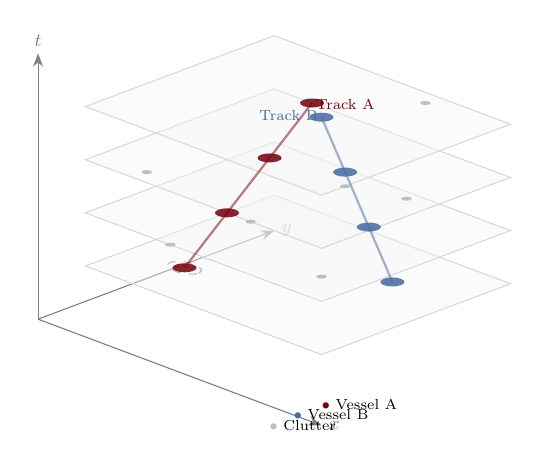
\begin{tikzpicture}[scale=0.75, transform shape,
    x={(0.8cm,-0.3cm)}, y={(0.8cm,0.3cm)}, z={(0cm,0.9cm)}]
    
    % Coordinate axes
    \draw[-{Stealth}, gray] (0,0,0) -- (6,0,0) node[right, font=\small] {$x$};
    \draw[-{Stealth}, gray] (0,0,0) -- (0,5,0) node[right, font=\small] {$y$};
    \draw[-{Stealth}, gray] (0,0,0) -- (0,0,5) node[above, font=\small] {$t$};
    
    % Time slice planes (semi-transparent)
    \foreach \z in {1,2,3,4} {
        \fill[gray!8, opacity=0.4] (0.5,0.5,\z) -- (5.5,0.5,\z) -- (5.5,4.5,\z) -- (0.5,4.5,\z) -- cycle;
        \draw[gray!30] (0.5,0.5,\z) -- (5.5,0.5,\z) -- (5.5,4.5,\z) -- (0.5,4.5,\z) -- cycle;
    }
    
    % Identity Tube 1 (garnet) - vessel moving diagonally
    \foreach \z in {1,2,3,4} {
        \pgfmathsetmacro{\xc}{1.2 + \z*0.4}
        \pgfmathsetmacro{\yc}{1.0 + \z*0.5}
        \fill[garnet, opacity=0.85] (\xc,\yc,\z) circle (0.18);
    }
    % Tube envelope
    \draw[garnet, thick, opacity=0.5] (1.6,1.5,1) -- (2.0,2.0,2) -- (2.4,2.5,3) -- (2.8,3.0,4);
    \draw[garnet, dashed, opacity=0.3] (1.6,1.5,1) ellipse (0.3 and 0.2);
    \node[garnet, font=\scriptsize] at (3.2,3.3,4) {Track A};
    
    % Identity Tube 2 (slate) - vessel moving opposite direction
    \foreach \z in {1,2,3,4} {
        \pgfmathsetmacro{\xc}{4.5 - \z*0.3}
        \pgfmathsetmacro{\yc}{3.5 - \z*0.2}
        \fill[slate, opacity=0.85] (\xc,\yc,\z) circle (0.18);
    }
    \draw[slate, thick, opacity=0.5] (4.2,3.3,1) -- (3.9,3.1,2) -- (3.6,2.9,3) -- (3.3,2.7,4);
    \node[slate, font=\scriptsize] at (2.9,2.4,4) {Track B};
    
    % Noise/clutter points (small, gray)
    \foreach \x/\y/\z in {1.0/3.5/1, 4.8/1.2/2, 2.5/4.0/2, 5.0/2.8/3, 1.5/0.8/3, 4.0/4.2/4, 0.8/2.0/1} {
        \fill[gray!50] (\x,\y,\z) circle (0.08);
    }
    
    % Legend
    \node[font=\scriptsize, align=left] at (5.8,1.0,0) {\textcolor{garnet}{$\bullet$} Vessel A};
    \node[font=\scriptsize, align=left] at (5.8,0.4,0) {\textcolor{slate}{$\bullet$} Vessel B};
    \node[font=\scriptsize, align=left] at (5.8,-0.2,0) {\textcolor{gray!50}{$\bullet$} Clutter};
\end{tikzpicture}
\end{document}
